\documentclass[11pt]{article}

% --- Paquetes ---
\usepackage[utf8]{inputenc}
\usepackage[T1]{fontenc}
\usepackage[spanish]{babel}
\usepackage{geometry}
\geometry{margin=2.5cm}
\usepackage{graphicx}
\usepackage{placeins}
\usepackage{booktabs}
\usepackage{amsmath}
\usepackage{amssymb}
\usepackage{threeparttable}
\usepackage{setspace}
\usepackage[backend=biber,style=authoryear]{biblatex}
\addbibresource{referencias.bib}

\onehalfspacing

% --- Información del documento ---
\title{\textbf{Tiempo de entrega y satisfacción del cliente en e-commerce:\\
una aplicación de regresión lineal múltiple y regresión logística}}
\author{Valeria Aranguren\\
Analítica de los Negocios\\
Pontificia Universidad Javeriana}
\date{Noviembre de 2026}

\begin{document}

\maketitle

\begin{abstract}
\noindent Este informe estudia la relación entre el tiempo de entrega y la
satisfacción del cliente en una plataforma de comercio electrónico, usando
113.559 pedidos entregados. Se estima una regresión lineal múltiple sobre la
calificación del cliente y un modelo logit sobre la probabilidad de una reseña
positiva. Los resultados muestran que lo que se asocia con la satisfacción no
es la duración prometida del envío, sino el cumplimiento de la promesa: cada
día adicional de retraso frente a la fecha estimada se asocia con 0,167
estrellas menos en la calificación y con una reducción de cerca del 47\% en
las probabilidades de una reseña positiva. Los resultados son asociaciones, no
efectos causales.
\end{abstract}

%=================================================================
\section{Introducción}
%=================================================================

En el comercio electrónico la entrega es uno de los pocos contactos tangibles
entre la plataforma y el cliente, y una parte grande de las quejas y
calificaciones gira alrededor de ella. Este informe responde una pregunta
concreta: ¿cómo se relaciona el tiempo de entrega, en particular la
diferencia entre la fecha prometida y la fecha real, con la satisfacción del
cliente, medida por su calificación y por el sentimiento de su reseña?

\subsection{Marco teórico}

La literatura reciente de operaciones y marketing ha estudiado esta relación
con datos de plataformas reales. \textcite{akturk2022} muestran, con datos de
una firma de e-commerce, que los tiempos de procesamiento y de entrega se
asocian con calificaciones más bajas, y que lo determinante es la desviación
entre la entrega real y la prometida: entregar tarde castiga la calificación y
entregar antes de lo prometido la mejora, con efectos curvilíneos.
\textcite{nozari2026} llegan a una conclusión similar con millones de compras:
las entregas tardías reducen las calificaciones de los productos, mientras que
las entregas tempranas tienen un efecto positivo menor. \textcite{ravula2023}
documenta que el castigo por entregar tarde es mayor que el premio por
entregar temprano, una asimetría consistente con la teoría de las
expectativas: el cliente compara lo recibido con lo prometido.

El desempeño logístico también tiene consecuencias comerciales más allá de la
calificación. \textcite{deshpande2023} conectan las métricas logísticas de una
plataforma con las calificaciones del servicio y con las ventas posteriores de
los vendedores. \textcite{rao2011} muestran que las fallas de cumplimiento de
los pedidos en línea se asocian con menores compras futuras, y
\textcite{harter2025} encuentran que los tiempos de entrega afectan la
recompra en el comercio rápido (\textit{quick commerce}).

Con base en esta literatura, el informe plantea dos ideas de trabajo:
(1) una mayor diferencia entre la entrega real y la prometida se asocia con
una menor calificación del cliente, y (2) esa misma diferencia se asocia con
una menor probabilidad de que la reseña sea positiva. Como los datos son
observacionales, los resultados se interpretan como asociaciones y no como
efectos causales.

%=================================================================
\section{Datos y análisis exploratorio}
%=================================================================

Los datos corresponden a 138.116 pedidos de una plataforma de comercio
electrónico, con 48 variables por pedido. La muestra de análisis se restringe
a los 113.559 pedidos efectivamente entregados: los 24.557 pedidos cancelados
o pendientes no tienen calificación, sentimiento ni tiempos de entrega, y se
excluyen del estudio.

Las variables del estudio son:

\begin{itemize}
    \item \textbf{Calificación del cliente} (\texttt{customer\_rating}):
    puntaje de 1 a 5 estrellas. Es la variable dependiente de la regresión
    lineal.
    \item \textbf{Sentimiento de la reseña} (\texttt{review\_sentiment}):
    clasificación de la reseña como positiva, neutral o negativa. Con ella se
    construye la variable binaria \texttt{sentimiento\_positivo}
    (1 = reseña positiva, 0 = neutral o negativa), que es la variable
    dependiente del modelo logit. Como las reseñas explícitamente negativas
    son apenas el 0,6\% de la base, se tomó la decisión, documentada en los
    scripts, de agrupar las reseñas neutrales con las negativas en la
    categoría 0.
    \item \textbf{Diferencia de entrega} (\texttt{diferencia\_entrega}):
    días de entrega reales menos días de entrega estimados. Un valor positivo
    indica retraso frente a la promesa; es la variable independiente central.
    \item \textbf{Tiempo de entrega estimado}
    (\texttt{estimated\_delivery\_days}): la promesa de entrega en días.
    \item \textbf{Controles}: edad del cliente, género (referencia:
    \textit{Female}), tipo de cliente (referencia: \textit{Loyal}, la
    categoría más frecuente) y método de envío (referencia:
    \textit{Standard}).
\end{itemize}

\begin{table}[htbp]
\centering
\caption{Estadisticas descriptivas de las variables numericas del estudio}
\label{tab:descriptivas}
\begin{tabular}{lrrrrrrr}
\toprule
Variable & n & Faltantes & Media & Desv. est. & Min. & Mediana & Max. \\
\midrule
customer\_rating & 113559 & 24557 & 3.68 & 0.48 & 1.60 & 3.70 & 5.00 \\
delivery\_days & 113559 & 24557 & 4.56 & 2.81 & 0.00 & 4.00 & 14.00 \\
estimated\_delivery\_days & 113559 & 24557 & 4.30 & 2.59 & 0.00 & 4.00 & 10.00 \\
diferencia\_entrega & 113559 & 24557 & 0.26 & 1.12 & -2.00 & 0.00 & 4.00 \\
customer\_age & 138116 & 0 & 45.86 & 16.47 & 18.00 & 46.00 & 74.00 \\
\bottomrule
\end{tabular}
\end{table}


La calificación promedio es 3,68 estrellas con una desviación estándar de
0,48. El 63,3\% de los pedidos llega exactamente en la fecha prometida
(diferencia de entrega igual a cero), y los retrasos llegan hasta cuatro días.
En la muestra entregada, el 68,8\% de las reseñas es positivo, el 30,5\%
neutral y el 0,7\% negativo. La Figura \ref{fig:hist} muestra la distribución
de la calificación y la Figura \ref{fig:diferencia} la de la diferencia de
entrega. La Figura \ref{fig:ratingdif} es el hallazgo exploratorio central:
la calificación promedio cae de manera clara y casi monótona a medida que
aumenta el retraso frente a lo prometido, lo que anticipa el resultado de los
modelos.

\begin{figure}[htbp]
    \centering
    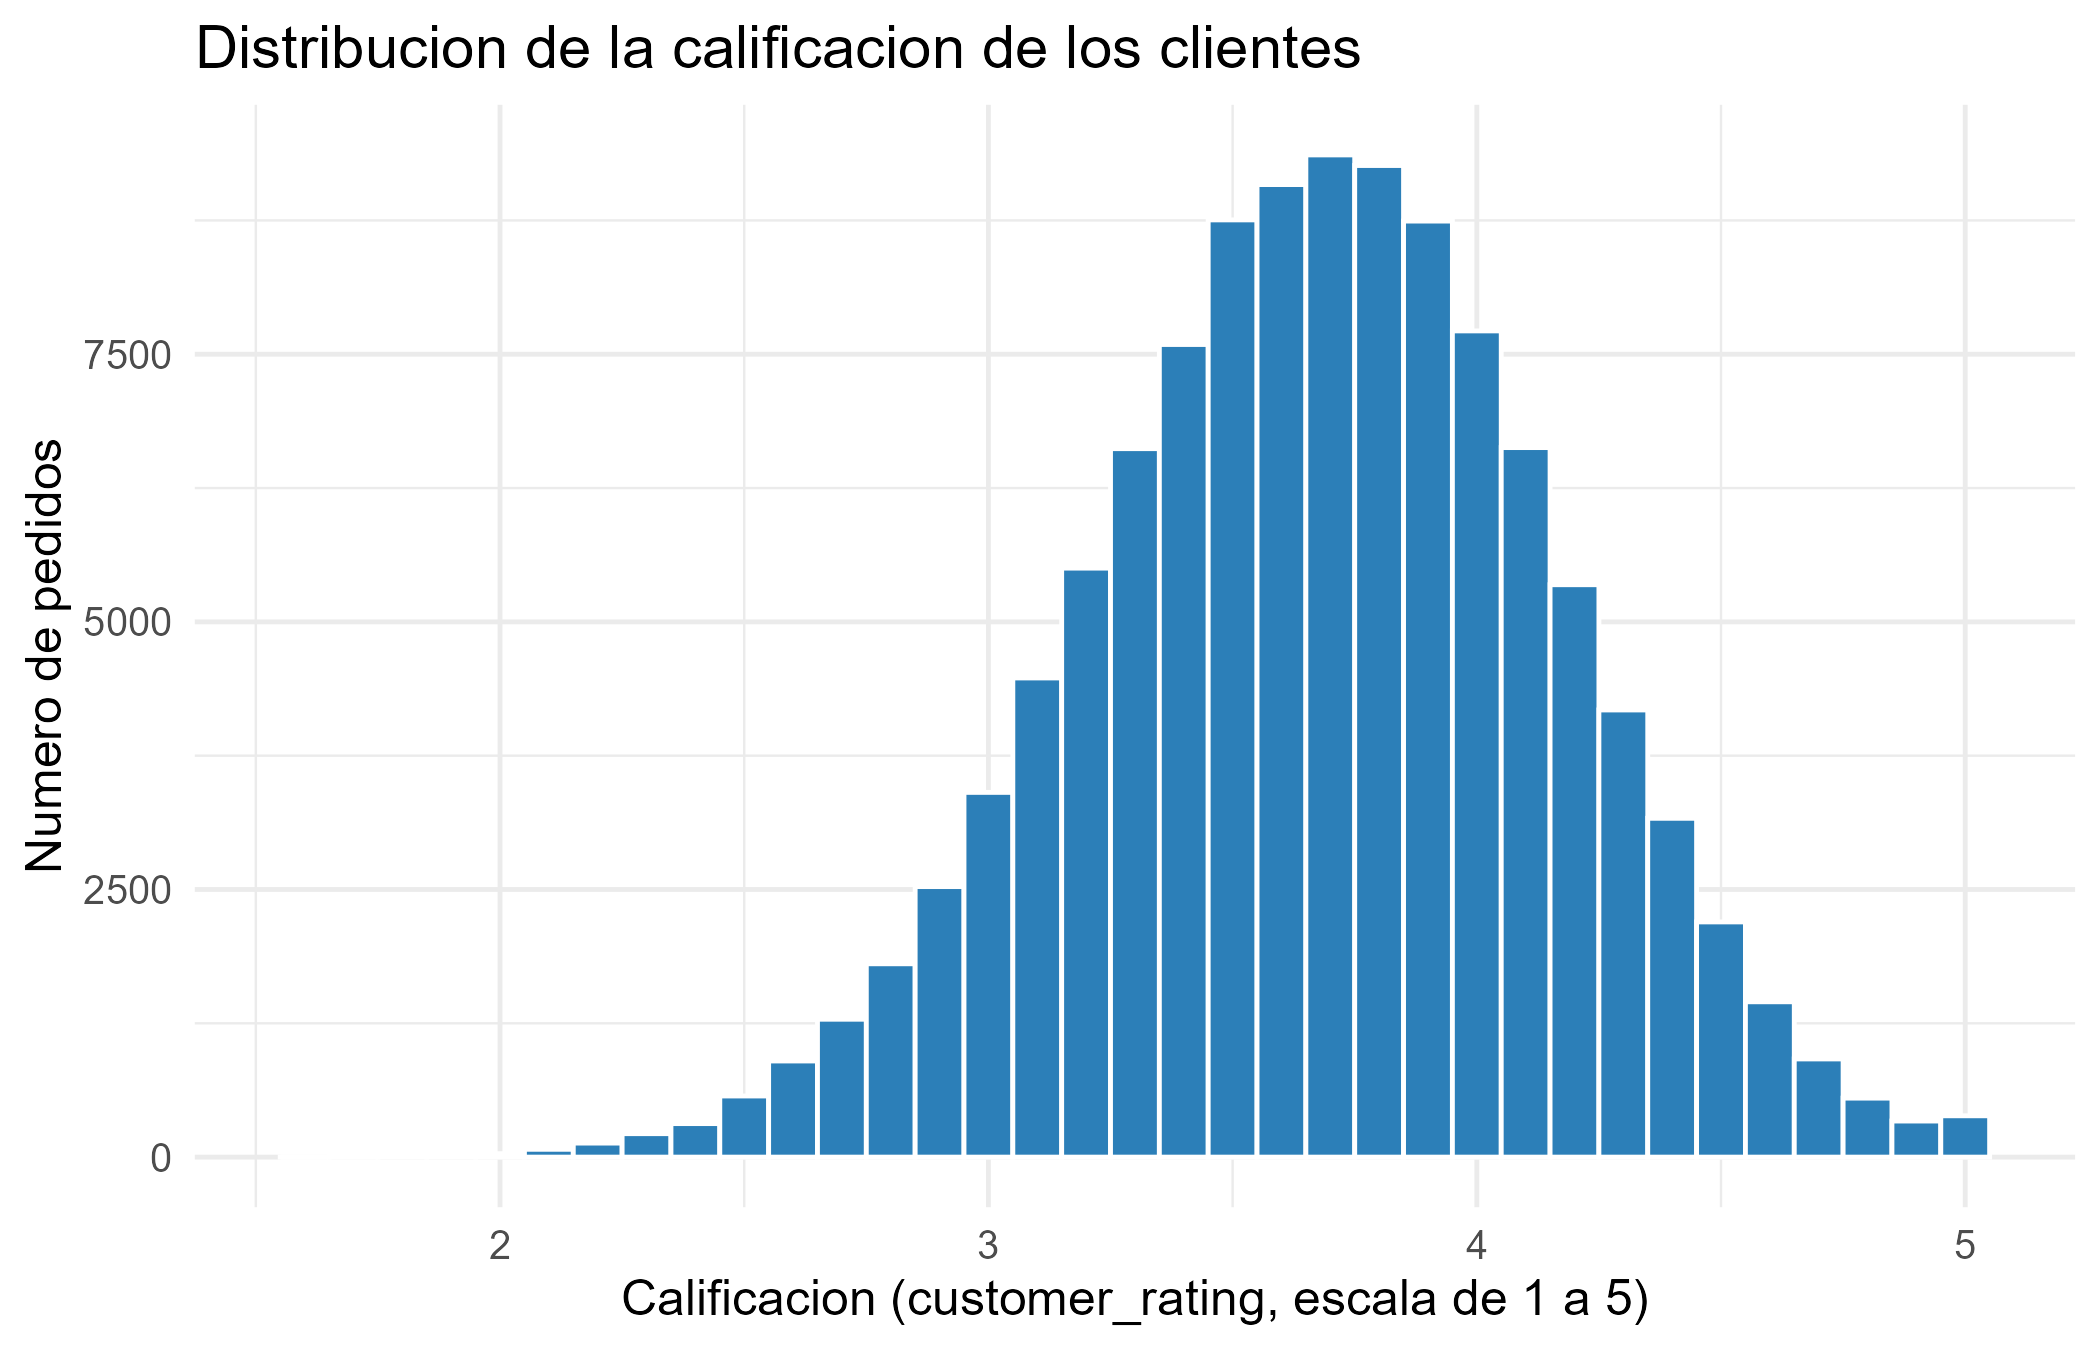
\includegraphics[width=0.75\textwidth]{salidas/figuras/fig_01_hist_rating.png}
    \caption{Distribución de la calificación del cliente}
    \label{fig:hist}
\end{figure}

\begin{figure}[htbp]
    \centering
    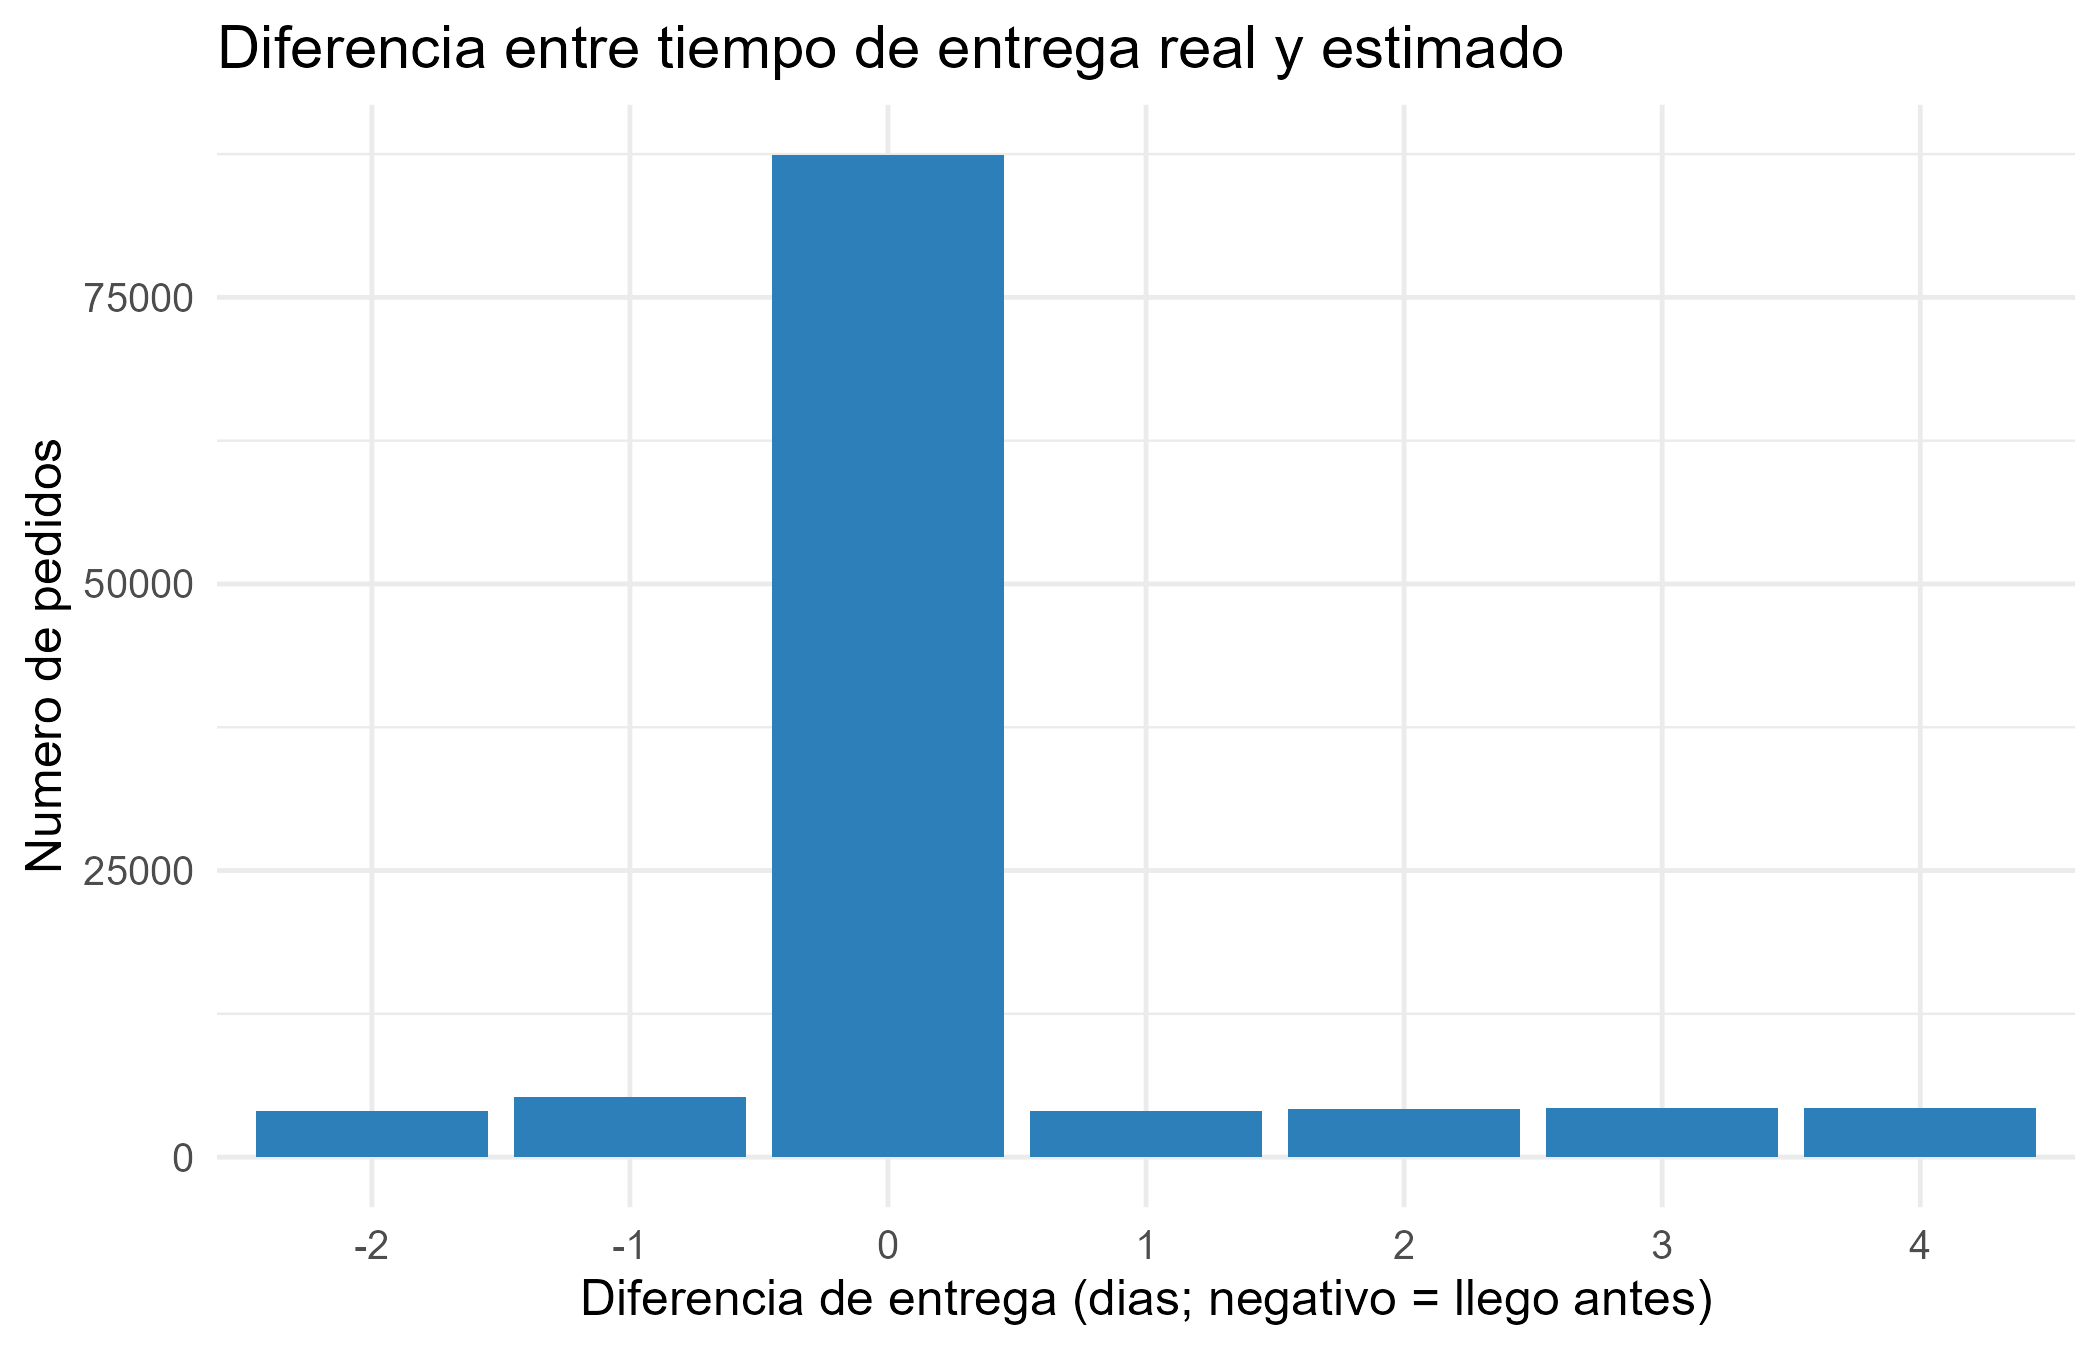
\includegraphics[width=0.75\textwidth]{salidas/figuras/fig_03_barras_diferencia.png}
    \caption{Distribución de la diferencia entre entrega real y prometida (días)}
    \label{fig:diferencia}
\end{figure}

\begin{figure}[htbp]
    \centering
    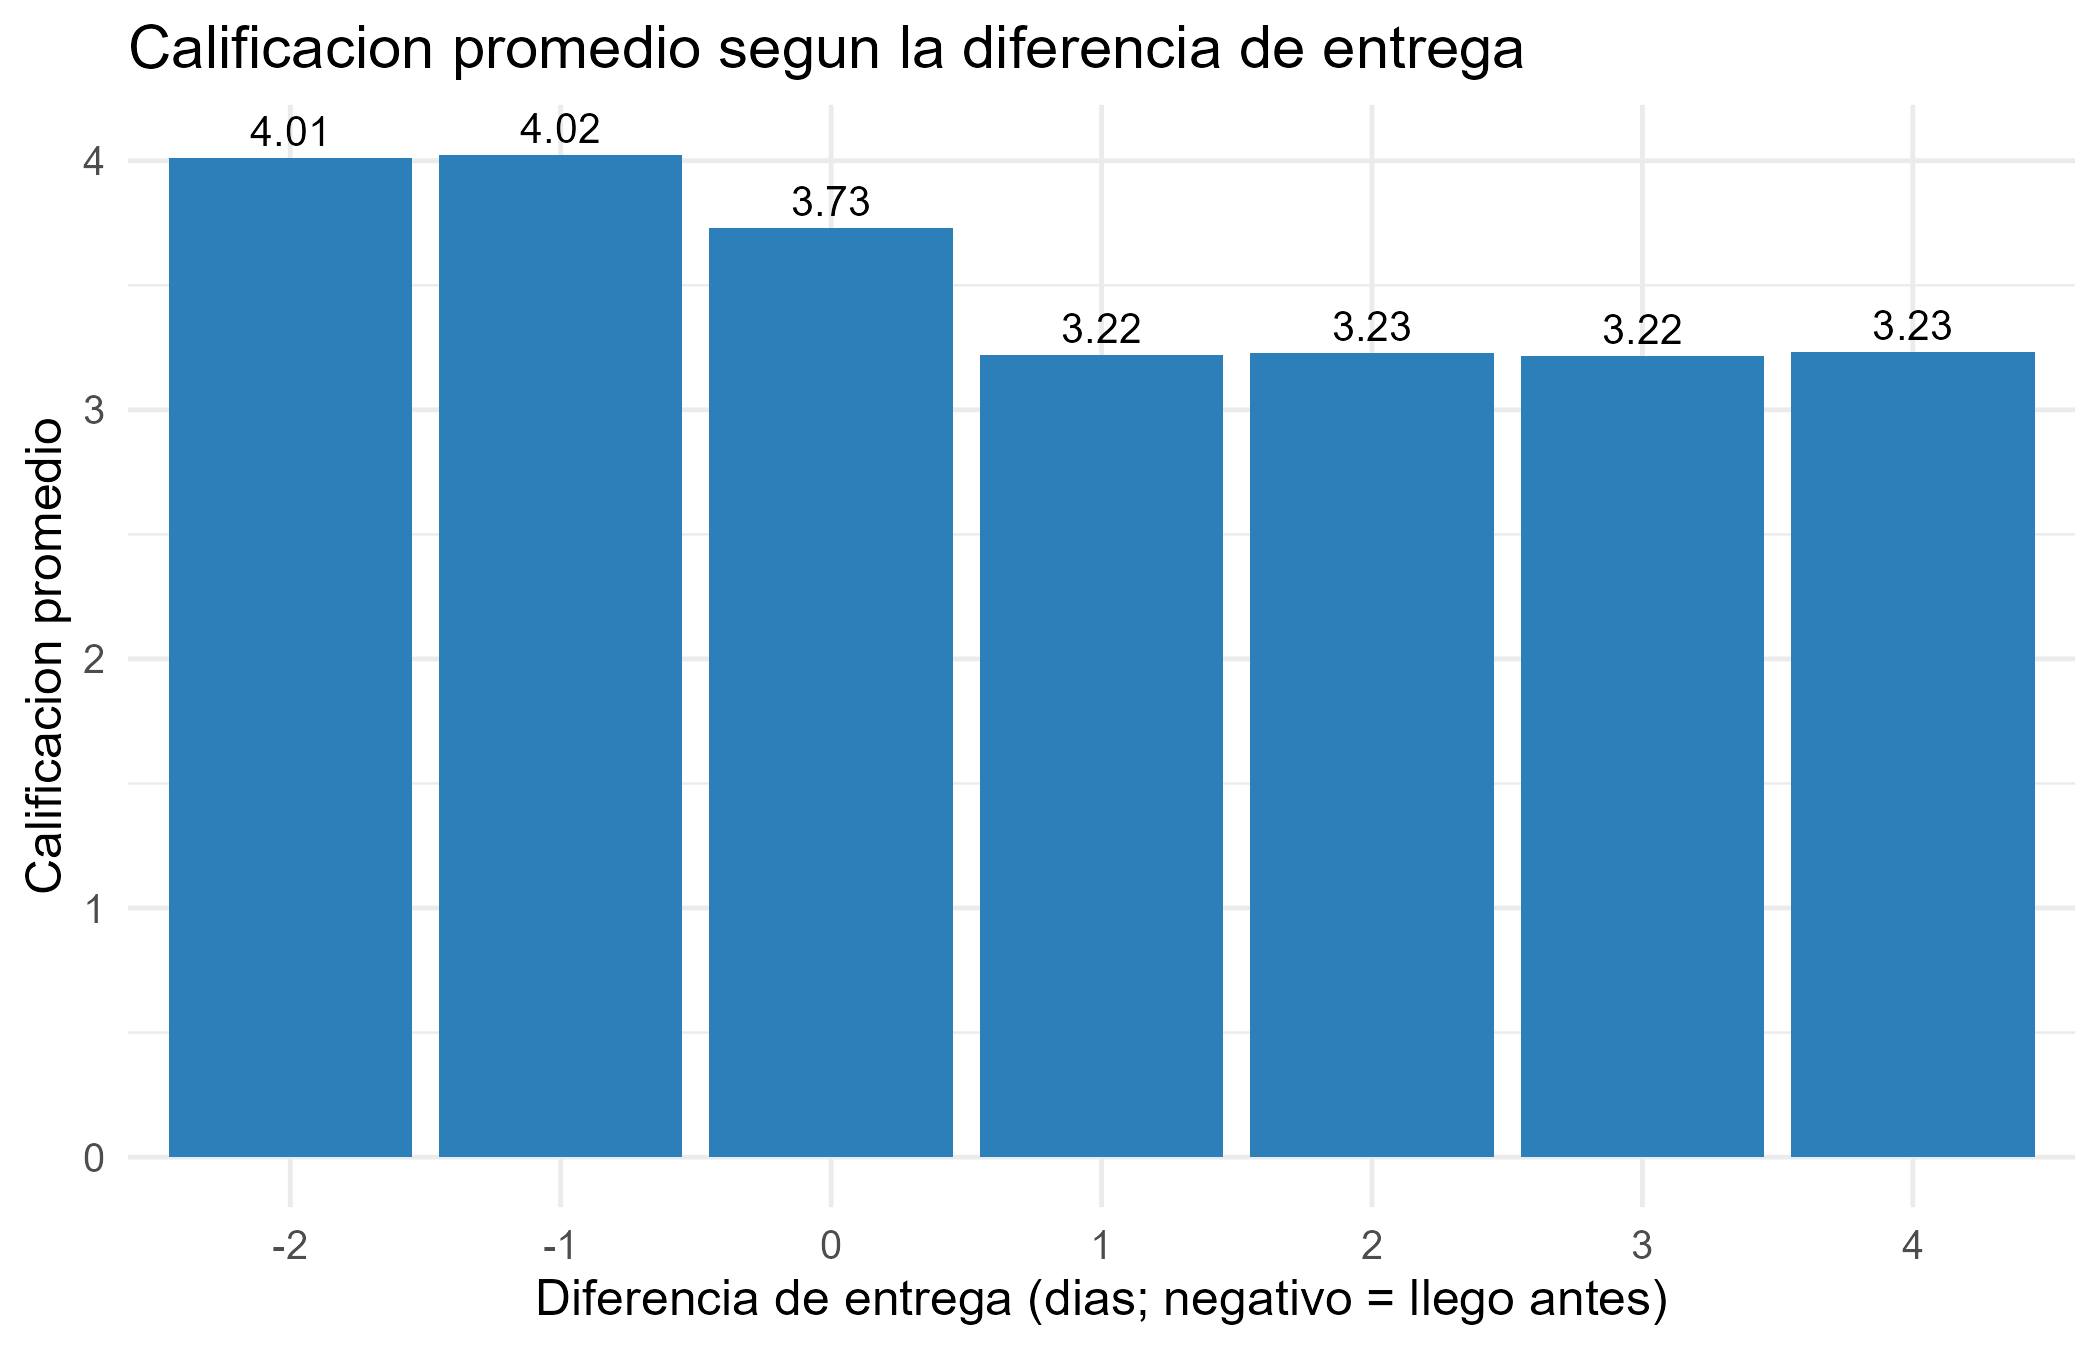
\includegraphics[width=0.8\textwidth]{salidas/figuras/fig_04_rating_por_diferencia.png}
    \caption{Calificación promedio según la diferencia de entrega}
    \label{fig:ratingdif}
\end{figure}

%=================================================================
\FloatBarrier
\section{Metodología}
%=================================================================

Se estiman dos modelos. El primero es una regresión lineal múltiple (MCO)
sobre la calificación:

\begin{equation}
\text{rating}_i = \beta_0 + \beta_1\,\text{diferencia\_entrega}_i
+ \beta_2\,\text{estimado}_i + \beta_3\,\text{edad}_i
+ \mathbf{\gamma}'\mathbf{X}_i + \varepsilon_i
\end{equation}

donde $\mathbf{X}_i$ incluye las variables dicotómicas de género, tipo de
cliente y método de envío (esquema $k-1$ con las categorías de referencia
indicadas). El coeficiente de interés es $\beta_1$: el cambio en la
calificación asociado con cada día adicional de retraso frente a la promesa.

El segundo es un modelo logit sobre la probabilidad de una reseña positiva:

\begin{equation}
\Pr(\text{sentimiento\_positivo}_i = 1) =
\Lambda\!\left(\beta_0 + \beta_1\,\text{diferencia\_entrega}_i
+ \beta_2\,\text{estimado}_i + \beta_3\,\text{edad}_i
+ \mathbf{\gamma}'\mathbf{X}_i\right)
\end{equation}

donde $\Lambda(\cdot)$ es la función logística. Para facilitar la
interpretación se reportan los \textit{odds ratios}, $\exp(\beta)$: valores
menores que uno indican una menor probabilidad de reseña positiva.

Como especificación de robustez, ambos modelos se reestiman reemplazando la
diferencia de entrega por la variable binaria \texttt{atrasado}, igual a 1 si
el pedido llegó después de la fecha prometida. Esta especificación capta el
efecto discreto de incumplir la promesa, que es lo que la literatura identifica
como lo más relevante \parencite{akturk2022,ravula2023}.

Dos limitaciones se tienen presentes en toda la interpretación. Primero, la
calificación está acotada entre 1 y 5 y aquí se trata como continua, lo que es
una primera aproximación razonable pero no la especificación ideal. Segundo,
los datos son observacionales: los coeficientes miden asociación, no
causalidad.

%=================================================================
\section{Resultados}
%=================================================================

\subsection{Regresión lineal múltiple}

\begin{table}[htbp]
\centering
\caption{Regresion lineal multiple: calificacion del cliente}
\label{tab:ols}
\begin{tabular}{lcc}
\toprule
Variable & Coeficiente & (Err. est.) \\
\midrule
(Intercept) & 3.727*** & (0.007) \\
diferencia\_entrega & -0.167*** & (0.001) \\
estimated\_delivery\_days & -0.002 & (0.001) \\
customer\_age & -0.000 & (0.000) \\
genderMale & -0.001 & (0.003) \\
genderNon-Binary & 0.011 & (0.007) \\
customer\_typeNew & -0.016 & (0.027) \\
customer\_typeReturning & -0.002 & (0.006) \\
shipping\_methodEconomy & -0.003 & (0.004) \\
shipping\_methodExpress & 0.002 & (0.005) \\
shipping\_methodSame Day & 0.010 & (0.007) \\
\bottomrule
\end{tabular}
\begin{minipage}{0.9\textwidth}\footnotesize Errores estandar entre parentesis. *** p$<$0.01, ** p$<$0.05, * p$<$0.1. \end{minipage}
\end{table}


El único coeficiente estadísticamente significativo es el de la diferencia de
entrega: $-0,167$ ($p<0{,}01$). Cada día adicional de retraso frente a la
fecha prometida se asocia con 0,167 estrellas menos en la calificación, una
magnitud considerable frente a la desviación estándar de la calificación
(0,48). Ni la duración de la promesa de entrega ni los controles demográficos
o de envío muestran una asociación significativa. El modelo explica el 14,9\%
de la variación de la calificación ($R^2 = 0{,}149$), un valor razonable para
datos individuales de este tipo.

\begin{table}[htbp]
\centering
\caption{Regresion lineal multiple: especificacion con atraso binario}
\label{tab:olsrob}
\begin{tabular}{lcc}
\toprule
Variable & Coeficiente & (Err. est.) \\
\midrule
(Intercept) & 3.764*** & (0.007) \\
atrasado & -0.531*** & (0.004) \\
estimated\_delivery\_days & -0.001 & (0.001) \\
customer\_age & -0.000 & (0.000) \\
genderMale & -0.001 & (0.003) \\
genderNon-Binary & 0.012* & (0.007) \\
customer\_typeNew & -0.010 & (0.027) \\
customer\_typeReturning & -0.003 & (0.006) \\
shipping\_methodEconomy & -0.003 & (0.004) \\
shipping\_methodExpress & 0.001 & (0.005) \\
shipping\_methodSame Day & -0.003 & (0.007) \\
\bottomrule
\end{tabular}
\begin{minipage}{0.9\textwidth}\footnotesize Errores estandar entre parentesis. *** p$<$0.01, ** p$<$0.05, * p$<$0.1. \end{minipage}
\end{table}


La especificación con atraso binario confirma el resultado: llegar tarde se
asocia con 0,531 estrellas menos en promedio ($p<0{,}01$), con un ajuste
ligeramente mejor ($R^2 = 0{,}153$). Es decir, lo que más se asocia con la
insatisfacción no es cuántos días tarde el envío en términos absolutos, sino
el hecho de incumplir la fecha prometida. 
\subsection{Modelo logit}

\begin{table}[htbp]
\centering
\caption{Modelo logit: probabilidad de resena positiva}
\label{tab:logit}
\begin{tabular}{lcc}
\toprule
Variable & Coeficiente & (Err. est.) \\
\midrule
(Intercept) & 1.035*** & (0.035) \\
diferencia\_entrega & -0.639*** & (0.007) \\
estimated\_delivery\_days & -0.005 & (0.005) \\
customer\_age & -0.000 & (0.000) \\
genderMale & -0.004 & (0.014) \\
genderNon-Binary & 0.035 & (0.036) \\
customer\_typeNew & -0.136 & (0.135) \\
customer\_typeReturning & -0.039 & (0.028) \\
shipping\_methodEconomy & -0.017 & (0.022) \\
shipping\_methodExpress & -0.000 & (0.023) \\
shipping\_methodSame Day & 0.016 & (0.033) \\
\bottomrule
\end{tabular}
\begin{minipage}{0.9\textwidth}\footnotesize Errores estandar entre parentesis. *** p$<$0.01, ** p$<$0.05, * p$<$0.1. \end{minipage}
\end{table}


\begin{table}[htbp]
\centering
\caption{Odds ratios del modelo logit}
\label{tab:logitor}
\begin{tabular}{lccc}
\toprule
Variable & Odds ratio & IC 95\% inf. & IC 95\% sup. \\
\midrule
(Intercept) & 2.815 & 2.630 & 3.013 \\
diferencia\_entrega & 0.528 & 0.521 & 0.535 \\
estimated\_delivery\_days & 0.995 & 0.984 & 1.005 \\
customer\_age & 1.000 & 0.999 & 1.001 \\
genderMale & 0.996 & 0.969 & 1.023 \\
genderNon-Binary & 1.036 & 0.965 & 1.112 \\
customer\_typeNew & 0.873 & 0.669 & 1.138 \\
customer\_typeReturning & 0.962 & 0.910 & 1.017 \\
shipping\_methodEconomy & 0.983 & 0.941 & 1.027 \\
shipping\_methodExpress & 1.000 & 0.955 & 1.046 \\
shipping\_methodSame Day & 1.016 & 0.952 & 1.085 \\
\bottomrule
\end{tabular}
\end{table}


En el modelo logit, el coeficiente de la diferencia de entrega es $-0,639$
($p<0{,}01$), con un \textit{odds ratio} de 0,528 (IC 95\%: 0,521-0,535): por
cada día adicional de retraso, las probabilidades (\textit{odds}) de que la
reseña sea positiva se reducen en cerca del 47\%. El pseudo $R^2$ de McFadden
es 0,083 y el porcentaje de aciertos del modelo es 73,2\%. De nuevo, la
duración prometida y los controles no son significativos.

\begin{table}[htbp]
\centering
\caption{Odds ratios del modelo logit (especificacion con atraso binario)}
\label{tab:logitorrob}
\begin{tabular}{lccc}
\toprule
Variable & Odds ratio & IC 95\% inf. & IC 95\% sup. \\
\midrule
(Intercept) & 3.196 & 2.985 & 3.423 \\
atrasado & 0.143 & 0.138 & 0.148 \\
estimated\_delivery\_days & 0.995 & 0.985 & 1.006 \\
customer\_age & 1.000 & 0.999 & 1.001 \\
genderMale & 0.996 & 0.969 & 1.023 \\
genderNon-Binary & 1.041 & 0.969 & 1.117 \\
customer\_typeNew & 0.887 & 0.680 & 1.157 \\
customer\_typeReturning & 0.957 & 0.905 & 1.012 \\
shipping\_methodEconomy & 0.982 & 0.940 & 1.027 \\
shipping\_methodExpress & 0.997 & 0.952 & 1.043 \\
shipping\_methodSame Day & 0.980 & 0.917 & 1.047 \\
\bottomrule
\end{tabular}
\end{table}


La robustez con la variable binaria es contundente: el \textit{odds ratio} de
\texttt{atrasado} es 0,143 (IC 95\%: 0,138-0,148), es decir, cuando el pedido
llega tarde las probabilidades de una reseña positiva son aproximadamente 86\%
menores. Este resultado es consistente con la asimetría documentada por
\textcite{ravula2023} y \textcite{nozari2026}: el incumplimiento de la promesa
pesa mucho más que cualquier otra característica del envío.


\subsection{Diagnóstico de los residuos}

La Figura \ref{fig:diag} reúne los cuatro gráficos de diagnóstico del modelo
de regresión lineal, que permiten revisar los supuestos de la estimación por
mínimos cuadrados ordinarios.

\begin{figure}[htbp]
    \centering
    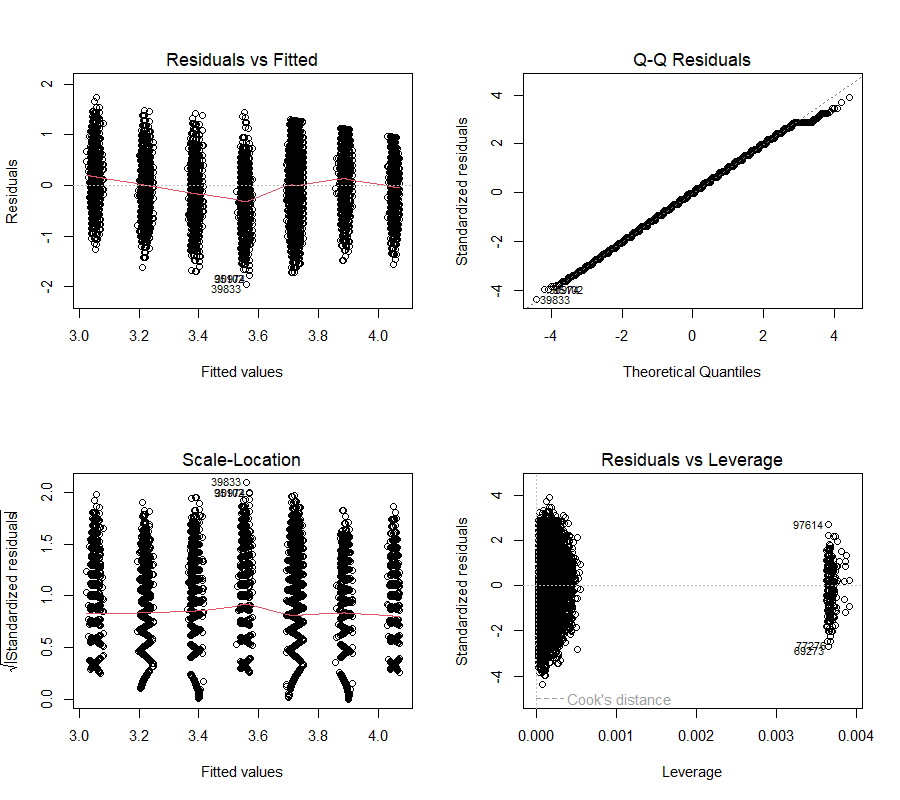
\includegraphics[width=0.85\textwidth]{salidas/figuras/diag_residuos_ols.png}
    \caption{Diagnóstico de residuos del modelo de regresión lineal}
    \label{fig:diag}
\end{figure}

En el gráfico de residuos frente a valores ajustados (\textit{Residuals vs
Fitted}), la línea suavizada roja se mantiene prácticamente plana alrededor de
cero en todo el rango de valores ajustados. No se observa una curva ni un
patrón sistemático en los residuos, lo que sugiere que la forma funcional
lineal es razonable para estos datos. Las columnas de puntos que se ven en el
gráfico no son un problema del modelo: aparecen porque la calificación solo
puede tomar valores enteros entre 1 y 5, de modo que los residuos se agrupan
en bandas discretas.

En cuanto a la heterocedasticidad, tanto en el gráfico de residuos frente a
valores ajustados como en el de escala-localización (\textit{Scale-Location})
la dispersión de los residuos es similar en todos los niveles de valores
ajustados y la línea suavizada es casi horizontal. No se ve el patrón de
embudo característico de la heterocedasticidad, por lo que la hipótesis de
varianza constante de los errores se sostiene razonablemente bien.

En el gráfico Q-Q, los residuos estandarizados siguen de cerca la línea
diagonal en casi todo el rango, con desviaciones leves en los extremos. Esto
indica que la distribución de los residuos es aproximadamente normal, con
colas un poco más pesadas que las de una normal perfecta, algo habitual cuando
la variable dependiente está acotada entre 1 y 5. Con una muestra de 113.559
observaciones, estas desviaciones menores no comprometen la validez de la
inferencia.

Por último, el gráfico de residuos frente a apalancamiento (\textit{Residuals
vs Leverage}) no muestra observaciones por fuera de las líneas de distancia de
Cook, es decir, ningún punto individual tiene una influencia desproporcionada
sobre los coeficientes estimados.

En conjunto, los diagnósticos no muestran problemas graves de especificación:
no hay evidencia de heterocedasticidad, los residuos son aproximadamente
normales y no aparece ningún patrón sistemático sin capturar. La principal
limitación sigue siendo la naturaleza acotada y discreta de la calificación,
que se traduce en las bandas visibles de los gráficos y que aconseja
interpretar los resultados como asociaciones promedio y no como efectos
causales.

%=================================================================
\section{Conclusiones}
%=================================================================

El análisis de 113.559 pedidos entregados muestra una relación clara y robusta
entre el cumplimiento de la promesa de entrega y la satisfacción del cliente.
Cada día de retraso frente a la fecha estimada se asocia con 0,167 estrellas
menos en la calificación y con una reducción cercana al 47\% en las
probabilidades de una reseña positiva; cuando el pedido llega tarde, esas
probabilidades caen cerca del 86\%. En cambio, la duración de la promesa en sí
no se asocia con la satisfacción: al cliente no le importa tanto cuánto se
demora el envío como que llegue cuando se le dijo.

Estos resultados están en línea con la literatura \parencite{akturk2022,
ravula2023, nozari2026} y tienen una implicación gerencial directa: más que
acortar los tiempos de entrega, la plataforma se beneficia de fijar promesas
realistas y cumplirlas.

Las conclusiones deben leerse con dos límites. Los resultados son
asociaciones y no prueban causalidad, y la calificación, acotada entre 1 y 5,
se trató como una variable continua. Como extensión natural queda estimar un
modelo ordenado para la calificación y explorar estrategias de identificación
causal, por ejemplo usando variación exógena en los tiempos de entrega.

%=================================================================
\printbibliography

\end{document}
